% !TeX root = ../main.tex

\newlecture[Markowitz Portfolio Theory][Nov 9, 2026]

\header{The Markowitz Model}
For a given mean return, you would like to \dbb{minimize your risk} (the variance).
\begin{center}
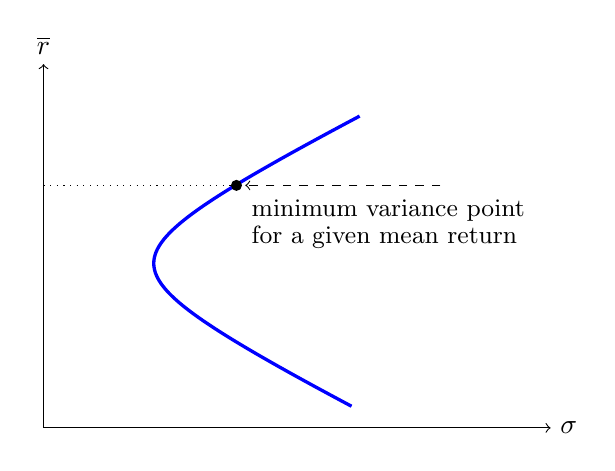
\begin{tikzpicture}[x=1.4cm, y=1.1cm]
    \draw[->] (0,0) -- (4.6,0) node[right] {$\sigma$};
    \draw[->] (0,0) -- (0,4.2) node[above] {$\overline{r}$};
    \draw[very thick, blue, domain=0.25:3.6, samples=60, smooth, variable=\r] plot ({sqrt(1 + 2.5*(\r-1.9)^2)}, {\r});
    \draw[dotted] (0,2.8) -- (1.75,2.8);
    \draw[->, dashed] (3.6,2.8) -- (1.83,2.8);
    \fill (1.75,2.8) circle (2pt);
    \node[below right, align=left] at (1.8,2.75) {\small minimum variance point\\[-2pt]\small for a given mean return};
\end{tikzpicture}
\end{center}
Markowitz formulated the problem of being on the efficient frontier as an \rb{optimization}. Assume there are $n$ \dbb{risky} assets with mean returns $\overline{r}_1, \overline{r}_2, \dots, \overline{r}_n$ and covariances $\sigma_{ij}$ for $i, j = 1, \dots, n$.

\begin{definition}[\rb{Markowitz Optimization}]
    \[\boxed{\begin{aligned}
        \text{minimize} &\quad \frac{1}{2}\sum_{i,j=1}^{n}w_iw_j\sigma_{ij} && = \tfrac{1}{2}(\text{variance})\\
        \text{subject to} &\quad \sum_{i=1}^{n}w_i\overline{r}_i = \overline{r}_p && = \text{target mean return}\\
        &\quad \sum_{i=1}^{n}w_i = 1 && = \text{weights sum to 1}
    \end{aligned}}\]
\end{definition}
\keypoint{Note: (1) we \rb{are} allowing short selling (no $w_i \geq 0$ constraint)! \quad (2) we assume \rb{all} assets are risky!}
The $\frac{1}{2}$ is only there to cancel the 2 when differentiating; it does not change the optimal $w$.

\header{Solving a General Optimization (Lagrange Multipliers)}
To solve
\[\min\ f(x,u) \qquad \text{s.t.}\quad g_1(x,u) = c_1, \quad g_2(x,u) = c_2\]
\begin{enumerate}[label=\textcolor{red!70!black}{\textbf{Step \arabic*:}}, leftmargin=*]
    \item Convert all constraints to have \dbb{zero on the right hand side}:
    \[g_1(x,u) - c_1 = 0, \qquad g_2(x,u) - c_2 = 0\]
    \item Associate a \rb{Lagrange multiplier} with each constraint:
    \[g_1(x,u) - c_1 = 0 \;\longleftarrow\; \lambda_1, \qquad g_2(x,u) - c_2 = 0 \;\longleftarrow\; \lambda_2\]
    \item Form the \rb{Lagrangian} by subtracting from the objective each constraint multiplied by its multiplier:
    \[\boxed{L(x,u,\lambda_1,\lambda_2) = f(x,u) - \lambda_1\left(g_1(x,u) - c_1\right) - \lambda_2\left(g_2(x,u) - c_2\right)}\]
    \item Compute the partial derivatives of $L$ with respect to \ul{all} its variables and set them equal to zero:
    \[\begin{aligned}
        \frac{\partial L}{\partial x} &= \frac{\partial f}{\partial x} - \lambda_1\frac{\partial g_1}{\partial x} - \lambda_2\frac{\partial g_2}{\partial x} = 0 & \qquad -\frac{\partial L}{\partial \lambda_1} &= g_1(x,u) - c_1 = 0\\
        \frac{\partial L}{\partial u} &= \frac{\partial f}{\partial u} - \lambda_1\frac{\partial g_1}{\partial u} - \lambda_2\frac{\partial g_2}{\partial u} = 0 & \qquad -\frac{\partial L}{\partial \lambda_2} &= g_2(x,u) - c_2 = 0
    \end{aligned}\]
    Note the derivatives with respect to the multipliers just give back the constraints.
    \item Solve these equations (for $x$, $u$, $\lambda_1$, $\lambda_2$) to find the optimal solution.
\end{enumerate}

\heading{Applying it to Markowitz}
\begin{enumerate}[label=\textcolor{red!70!black}{\textbf{Step \arabic*:}}, leftmargin=*]
    \item Zero right hand sides, and
    \item a multiplier for each constraint ($\lambda$ for return, $\mu$ for budget):
    \[\min\ \frac{1}{2}\sum_{i,j=1}^{n}w_iw_j\sigma_{ij} \quad \text{s.t.}\quad \sum_{i=1}^{n}w_i\overline{r}_i - \overline{r}_p = 0 \;\longleftarrow\; \lambda, \qquad \sum_{i=1}^{n}w_i - 1 = 0 \;\longleftarrow\; \mu\]
    \setcounter{enumi}{2}
    \item Form the Lagrangian:
    \[L(w,\lambda,\mu) = \frac{1}{2}\sum_{i,j=1}^{n}w_iw_j\sigma_{ij} - \lambda\left(\sum_{i=1}^{n}w_i\overline{r}_i - \overline{r}_p\right) - \mu\left(\sum_{i=1}^{n}w_i - 1\right)\]
    \item Differentiate with respect to $w_i$, $\lambda$, $\mu$ and set to zero. ($w_i$ appears in the double sum once as $w_i$ and once as $w_j$, and $\sigma_{ij} = \sigma_{ji}$, so the $\frac{1}{2}$ cancels.)
    \[\boxed{\begin{aligned}
        w_i:&\quad \sum_{j=1}^{n}\sigma_{ij}w_j - \lambda\overline{r}_i - \mu = 0 \qquad \text{for } i = 1, \dots, n\\
        \lambda:&\quad \sum_{i=1}^{n}w_i\overline{r}_i = \overline{r}_p\\
        \mu:&\quad \sum_{i=1}^{n}w_i = 1
    \end{aligned}}\]
    \item Solve to obtain the optimal weights: \dbb{$n+2$ equations, $n+2$ unknowns} ($w_1, \dots, w_n, \lambda, \mu$).
\end{enumerate}
\keypoint{These equations \rb{characterize efficient funds}: any portfolio that satisfies them (for some $\lambda, \mu$) is on the minimum-variance set.}

\begin{example}[A Three-Asset Markowitz Example]
    $\overline{r}_1 = 0.05$, $\overline{r}_2 = 0.10$, $\overline{r}_3 = 0.15$, target $\overline{r}_p = 0.1125$. All assets risky, short selling allowed. Covariances:
    \begin{center}
    \begin{tabular}{cccc}
        \toprule
        $\sigma_{ij}$ & Asset 1 & Asset 2 & Asset 3\\
        \midrule
        Asset 1 & 0.05 & 0.01 & 0.01\\
        Asset 2 & 0.01 & 0.07 & 0.01\\
        Asset 3 & 0.01 & 0.01 & 0.05\\
        \bottomrule
    \end{tabular}
    \end{center}
    Find the minimum-variance portfolio with expected return 11.25\%.

    \b{Steps 1--2} (objective and constraints). Each cross term appears \dbb{twice} in the double sum ($\sigma_{12}w_1w_2$ and $\sigma_{21}w_2w_1$), so $0.01 + 0.01 = 0.02$:
    \begin{align*}
        \min\ \frac{1}{2}\sum_{i,j=1}^{3}w_iw_j\sigma_{ij} &= \frac{1}{2}\big(0.05w_1^2 + 0.07w_2^2 + 0.05w_3^2\\
        &\qquad\quad + 0.02w_1w_2 + 0.02w_1w_3 + 0.02w_2w_3\big)\\[4pt]
        \text{s.t.}\quad 0.05w_1 + 0.10w_2 + 0.15w_3 - 0.1125 &= 0 \;\longleftarrow\; \lambda\\
        w_1 + w_2 + w_3 - 1 &= 0 \;\longleftarrow\; \mu
    \end{align*}

    \b{Step 3} (Lagrangian):
    \begin{align*}
        L(w,\lambda,\mu) = {} & \tfrac{1}{2}\left(0.05w_1^2 + 0.07w_2^2 + 0.05w_3^2 + 0.02w_1w_2 + 0.02w_1w_3 + 0.02w_2w_3\right)\\
        & - \lambda\left(0.05w_1 + 0.10w_2 + 0.15w_3 - 0.1125\right) - \mu\left(w_1 + w_2 + w_3 - 1\right)
    \end{align*}

    \b{Step 4} (all five derivatives $= 0$): three stationarity equations (one per weight, each row of $\Sigma$) and two feasibility equations:
    \begin{align}
        0.05w_1 + 0.01w_2 + 0.01w_3 - 0.05\lambda - \mu &= 0 \tag{1}\\
        0.01w_1 + 0.07w_2 + 0.01w_3 - 0.10\lambda - \mu &= 0 \tag{2}\\
        0.01w_1 + 0.01w_2 + 0.05w_3 - 0.15\lambda - \mu &= 0 \tag{3}\\
        0.05w_1 + 0.10w_2 + 0.15w_3 &= 0.1125 \tag{4}\\
        w_1 + w_2 + w_3 &= 1 \tag{5}
    \end{align}
    Five equations, five unknowns: three weights, $\lambda$, and $\mu$.

    \b{Step 5} (solve). First eliminate $\mu$ by subtracting: (2)$-$(1) and (3)$-$(2):
    \[-0.04w_1 + 0.06w_2 = 0.05\lambda, \qquad -0.06w_2 + 0.04w_3 = 0.05\lambda\]
    Both equal $0.05\lambda$, so set them equal (this eliminates $\lambda$) and use (5):
    \[0.12w_2 = 0.04(w_1 + w_3) = 0.04(1 - w_2) \quad \Rightarrow \quad w_2 = 0.25, \quad w_1 + w_3 = 0.75\]
    Subtract $0.10\times$(5) from (4):
    \[-0.05w_1 + 0.05w_3 = 0.0125 \quad \Rightarrow \quad w_3 - w_1 = 0.25\]
    \[\boxed{w_1 = 0.25, \quad w_2 = 0.25, \quad w_3 = 0.50}\]
    Recover the multipliers by substituting back:
    \begin{align*}
        0.05\lambda &= -0.04(0.25) + 0.06(0.25) = 0.005 \quad \Rightarrow \quad \lambda = 0.10\\
        \mu &= 0.05(0.25) + 0.01(0.25) + 0.01(0.50) - 0.05(0.10) = 0.015
    \end{align*}
    Check (2) and (3): $0.025 - 0.10(0.10) - 0.015 = 0$ and $0.030 - 0.15(0.10) - 0.015 = 0$. \checkmark

    \b{Result}: 25\% in asset 1, 25\% in asset 2, 50\% in asset 3.
    \begin{align*}
        \overline{r}_p &= 0.25(0.05) + 0.25(0.10) + 0.50(0.15) = 0.1125 \quad \text{(meets the target)}\\
        \sigma_p^2 &= w^T\Sigma w = 0.25(0.020) + 0.25(0.025) + 0.50(0.030) = 0.02625
    \end{align*}
    Here $(0.020, 0.025, 0.030) = \Sigma w$, the first three terms of (1)--(3). So $\sigma_p = \sqrt{0.02625} \approx 0.162$ (16.20\%), and the minimized objective is $\frac{1}{2}\sigma_p^2 = 0.013125$.

    \b{Why is this the unique minimum?} $\Sigma$ is positive definite, so the objective is \dbb{strictly convex}. The feasible stationary point is therefore the unique global minimizer.
\end{example}

\header{The Two-Fund Theorem}
Assumptions:
\begin{enumerate}[label=(\arabic*)]
    \item Short selling is allowed.
    \item All assets are risky.
    \item All investors have the same estimates of means, variances, and covariances.
\end{enumerate}
\begin{framed}
    \textbf{Theorem} (\rb{Two-Fund Theorem}). Investors seeking efficient (minimum variance) portfolios need only invest in \dbb{combinations of two efficient funds}.
\end{framed}
\keypoint{Only two efficient funds need to exist, and everyone can invest in them!}
\begin{center}
\begin{tikzpicture}[x=1.4cm, y=1.1cm]
    \draw[->] (0,0) -- (4.6,0) node[right] {$\sigma$};
    \draw[->] (0,0) -- (0,4.2) node[above] {$\overline{r}$};
    \draw[thick, domain=0.25:3.8, samples=60, smooth, variable=\r] plot ({sqrt(1 + 2.5*(\r-1.9)^2)}, {\r});
    \foreach \r/\lab/\c/\pos in {2.3/{Fund 1}/blue/right, 3.4/{Fund 2}/blue/right, 2.85/{another efficient fund}/red/left} {
        \pgfmathsetmacro{\s}{sqrt(1 + 2.5*(\r-1.9)^2)}
        \fill[\c] (\s,\r) circle (2.2pt) node[\pos, black] {\small \lab};
    }
\end{tikzpicture}
\end{center}
The red fund is \ul{just a portfolio of Fund 1 and Fund 2}.

\heading{Proof}
Let $(\overline{r}_P^1, \lambda^1, \mu^1, w^1)$ and $(\overline{r}_P^2, \lambda^2, \mu^2, w^2)$ be efficient funds, so each satisfies the efficient-fund equations:
\[\begin{array}{c|c}
    \textcolor{red!70!black}{\textbf{1:}} & \textcolor{red!70!black}{\textbf{2:}}\\[2pt]
    \displaystyle\sum_{j=1}^{n}\sigma_{ij}w_j^1 - \lambda^1\overline{r}_i - \mu^1 = 0 & \displaystyle\sum_{j=1}^{n}\sigma_{ij}w_j^2 - \lambda^2\overline{r}_i - \mu^2 = 0\\[10pt]
    \displaystyle\sum_{i=1}^{n}w_i^1\overline{r}_i = \overline{r}_P^1, \quad \sum_{i=1}^{n}w_i^1 = 1 & \displaystyle\sum_{i=1}^{n}w_i^2\overline{r}_i = \overline{r}_P^2, \quad \sum_{i=1}^{n}w_i^2 = 1
\end{array}\]
Now consider an efficient fund with mean return $\overline{r}_P^3$. Solve $\alpha\overline{r}_P^1 + (1-\alpha)\overline{r}_P^2 = \overline{r}_P^3$ for $\alpha$ and set
\[w^3 = \alpha w^1 + (1-\alpha)w^2, \qquad \lambda^3 = \alpha\lambda^1 + (1-\alpha)\lambda^2, \qquad \mu^3 = \alpha\mu^1 + (1-\alpha)\mu^2\]
Are these the optimal weights and multipliers for $\overline{r}_P^3$? Yes! We show they satisfy all three equations for fund 3:
\begin{itemize}
    \item \b{Stationarity}:
    \begin{align*}
        \sum_{j=1}^{n}\sigma_{ij}w_j^3 - \lambda^3\overline{r}_i - \mu^3 &= \sum_{j=1}^{n}\sigma_{ij}\left(\alpha w_j^1 + (1-\alpha)w_j^2\right)\\
        &\qquad - \left(\alpha\lambda^1 + (1-\alpha)\lambda^2\right)\overline{r}_i - \left(\alpha\mu^1 + (1-\alpha)\mu^2\right)\\
        &= \alpha\underbrace{\left(\sum_{j=1}^{n}\sigma_{ij}w_j^1 - \lambda^1\overline{r}_i - \mu^1\right)}_{=\,0 \text{ by } 1} + (1-\alpha)\underbrace{\left(\sum_{j=1}^{n}\sigma_{ij}w_j^2 - \lambda^2\overline{r}_i - \mu^2\right)}_{=\,0 \text{ by } 2} = 0
    \end{align*}
    \item \b{Mean return}:
    \[\sum_{i=1}^{n}w_i^3\overline{r}_i = \alpha\left(\sum_{i=1}^{n}w_i^1\overline{r}_i\right) + (1-\alpha)\left(\sum_{i=1}^{n}w_i^2\overline{r}_i\right) = \alpha\overline{r}_P^1 + (1-\alpha)\overline{r}_P^2 = \overline{r}_P^3\]
    \item \b{Budget}:
    \[\sum_{i=1}^{n}w_i^3 = \alpha\left(\sum_{i=1}^{n}w_i^1\right) + (1-\alpha)\left(\sum_{i=1}^{n}w_i^2\right) = \alpha + (1-\alpha) = 1\]
\end{itemize}
So $(w^3, \lambda^3, \mu^3)$ \rb{is efficient}! The key is that all the efficient-fund equations are \dbb{linear} in $(w, \lambda, \mu)$, so combinations of solutions are solutions. \hfill$\blacksquare$

\begin{example}[Two-Fund Theorem]
    A market has 3 risky assets. Two efficient funds are
    \[w_A = \begin{bmatrix}0.25\\ 0.25\\ 0.50\end{bmatrix} \text{ with } \mu_A = 10\%, \qquad w_B = \begin{bmatrix}0.10\\ 0.70\\ 0.20\end{bmatrix} \text{ with } \mu_B = 20\%\]
    What are the weights of the efficient portfolio with mean return (a) 15\%, (b) 30\%?

    By the Two-Fund Theorem, $w_C = \alpha w_A + (1-\alpha)w_B$ for some $\alpha$. Find $\alpha$ by matching the mean return, $\alpha\mu_A + (1-\alpha)\mu_B = \mu_C$.
    \begin{enumerate}[label=(\alph*)]
        \item $0.10\alpha + 0.20(1-\alpha) = 0.15 \Rightarrow \alpha = 0.5$:
        \[w_C = 0.5\begin{bmatrix}0.25\\ 0.25\\ 0.50\end{bmatrix} + 0.5\begin{bmatrix}0.10\\ 0.70\\ 0.20\end{bmatrix} = \begin{bmatrix}0.175\\ 0.475\\ 0.350\end{bmatrix}\]
        \item $0.10\alpha + 0.20(1-\alpha) = 0.30 \Rightarrow \alpha = -1$, so $w_C = -w_A + 2w_B$:
        \[w_C = -\begin{bmatrix}0.25\\ 0.25\\ 0.50\end{bmatrix} + 2\begin{bmatrix}0.10\\ 0.70\\ 0.20\end{bmatrix} = \begin{bmatrix}-0.05\\ 1.15\\ -0.10\end{bmatrix}\]
        $\alpha < 0$ means \dbb{shorting fund A}, so the result shorts assets 1 and 3. That's allowed, since the theorem assumes short selling.
    \end{enumerate}
    In both cases the weights sum to 1.
\end{example}

\header{Inclusion of a Risk-Free Asset}
So far all assets were risky. Now assume there is also a \rb{risk-free asset} with return $r_f$ (so $\sigma = 0$). Combine it with a risky portfolio:
\[\text{risk free: } (r_f, 0) \qquad \text{risky asset: } (\overline{r}, \sigma^2)\]
Form a portfolio with $\alpha$ of the risk-free asset and $1-\alpha$ of the risky asset. Using the variance trick, $\operatorname{var}(\alpha r_f + (1-\alpha)r) = (1-\alpha)^2\sigma^2$, since $r_f$ is a constant:
\keypoint{mean: $\alpha r_f + (1-\alpha)\overline{r}$ \qquad variance: $(1-\alpha)^2\sigma^2$ \qquad standard deviation: $(1-\alpha)\sigma$}
As we vary $\alpha$, $(\sigma, \overline{r}) = \left((1-\alpha)\sigma,\ \alpha r_f + (1-\alpha)\overline{r}\right)$ traces a \rb{straight line} from $(0, r_f)$ through the risky asset:
\begin{center}
\begin{tikzpicture}[x=1.4cm, y=1.1cm]
    \draw[->] (0,0) -- (4.6,0) node[right] {$\sigma$};
    \draw[->] (0,0) -- (0,4.2) node[above] {$\overline{r}$};
    \draw[thick, domain=0.25:3.8, samples=60, smooth, variable=\r] plot ({sqrt(1 + 2.5*(\r-1.9)^2)}, {\r});
    \draw (0.08,1.2) -- (-0.08,1.2) node[left] {$r_f$};
    \pgfmathsetmacro{\s}{sqrt(1 + 2.5*(2.6-1.9)^2)}
    \draw[very thick, ->] (0,1.2) -- ({4.4},{1.2 + 4.4*(2.6-1.2)/\s});
    \fill (\s,2.6) circle (2pt) node[below right] {\small $(\overline{r}, \sigma^2)$};
\end{tikzpicture}
\end{center}
$\alpha = 1$ is all risk-free (on the axis), $\alpha = 0$ is all risky, and $\alpha < 0$ (borrowing at $r_f$) extends the line beyond the risky point.

\heading{Expanded Feasible Region}
Doing this for every risky portfolio fills the region between two lines from $r_f$. The upper line is \dbb{tangent} to the risky feasible region at the fund $F$:
\begin{center}
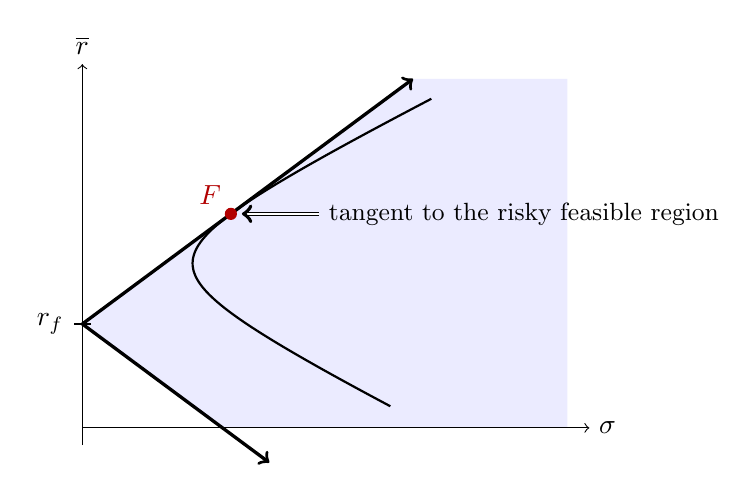
\begin{tikzpicture}[x=1.4cm, y=1.1cm]
    % tangency for sigma^2 = 1 + 2.5(r-1.9)^2 from r_f = 1.2: slope sqrt(0.49+0.4)
    \pgfmathsetmacro{\m}{sqrt(0.49 + 0.4)}
    \pgfmathsetmacro{\rT}{1.9 + 1/(2.5*0.7)}
    \pgfmathsetmacro{\sT}{sqrt(1 + 2.5*(\rT-1.9)^2)}
    \fill[blue!8] (0,1.2) -- (3.0,{1.2 + 3.0*\m}) -- (4.4,{1.2 + 3.0*\m}) -- (4.4,0) -- ({1.2/\m},0) -- cycle;
    \draw[->] (0,0) -- (4.6,0) node[right] {$\sigma$};
    \draw[->] (0,-0.2) -- (0,4.2) node[above] {$\overline{r}$};
    \draw[thick, domain=0.25:3.8, samples=60, smooth, variable=\r] plot ({sqrt(1 + 2.5*(\r-1.9)^2)}, {\r});
    \draw (0.08,1.2) -- (-0.08,1.2) node[left] {$r_f$};
    \draw[very thick, ->] (0,1.2) -- (3.0,{1.2 + 3.0*\m});
    \draw[very thick, ->] (0,1.2) -- ({1.6/\m},-0.4);
    \fill[red!70!black] (\sT,\rT) circle (2.2pt) node[above left] {$F$};
    \draw[<-, double] ({\sT+0.1},\rT) -- ({\sT+0.8},\rT) node[right] {\small tangent to the risky feasible region};
\end{tikzpicture}
\end{center}
The lower line comes from \ul{shorting} $F$ to invest more in the risk-free asset ($\alpha > 1$): the risk is $|1-\alpha|\sigma_F$, but the mean drops below $r_f$.

\header{The One-Fund Theorem}
Assumptions:
\begin{enumerate}[label=(\arabic*)]
    \item Short selling is allowed.
    \item There is a risk-free asset.
    \item All investors have the same estimates of means, variances, and covariances.
\end{enumerate}
\begin{framed}
    \textbf{Theorem} (\rb{One-Fund Theorem}). There is a \dbb{single fund $F$} of risky assets such that any efficient portfolio can be constructed as a combination of the fund $F$ and the risk-free asset.
\end{framed}
The efficient frontier is now the \ul{upper straight line} from $r_f$ through $F$. Every investor holds the same risky fund $F$. Investors differ only in how they split money between $F$ and the risk-free asset (more risk-averse means more in $r_f$).

\heading{Computation of the One-Fund}
The one-fund is the fund of risky assets with the \rb{maximum slope} from the risk-free rate:
\[\text{slope} = \frac{\overline{r}_{\text{Fund}} - r_f}{\sigma_{\text{Fund}}} = \max_{w}\ \frac{\displaystyle\sum_{i=1}^{n}w_i(\overline{r}_i - r_f)}{\displaystyle\left(\sum_{i,j=1}^{n}w_iw_j\sigma_{ij}\right)^{1/2}}\]
(Since $\sum w_i = 1$, the numerator is $\sum w_i\overline{r}_i - r_f$.) Take the derivative with respect to $w_k$, $k = 1, \dots, n$, using the quotient rule, and set it to zero:
\[\frac{\displaystyle\left(\sum_{i,j}w_iw_j\sigma_{ij}\right)^{1/2}(\overline{r}_k - r_f) - \left(\sum_{i}w_i(\overline{r}_i - r_f)\right)\left(\sum_{i,j}w_iw_j\sigma_{ij}\right)^{-1/2}\left(\sum_{j}w_j\sigma_{kj}\right)}{\displaystyle\sum_{i,j}w_iw_j\sigma_{ij}} = 0\]
Multiply through by $\left(\sum_{i,j}w_iw_j\sigma_{ij}\right)^{1/2}$:
\[(\overline{r}_k - r_f) - \frac{\left(\sum_{i}w_i(\overline{r}_i - r_f)\right)\left(\sum_{j}w_j\sigma_{kj}\right)}{\sum_{i,j}w_iw_j\sigma_{ij}} = 0\]
Let $\lambda = \dfrac{\sum_{i}w_i(\overline{r}_i - r_f)}{\sum_{i,j}w_iw_j\sigma_{ij}}$ (a single number, the same for every $k$). Then
\[(\overline{r}_k - r_f) - \lambda\sum_{j=1}^{n}w_j\sigma_{kj} = 0 \quad \Rightarrow \quad \sum_{j=1}^{n}\lambda w_j\sigma_{kj} = \overline{r}_k - r_f \qquad \text{for } k = 1, \dots, n\]
Let $v_j = \lambda w_j$:
\[\boxed{\sum_{j=1}^{n}\sigma_{kj}v_j = \overline{r}_k - r_f \quad \text{for } k = 1, \dots, n \qquad \Longrightarrow \qquad w_j = \frac{v_j}{\sum_{i=1}^{n}v_i}}\]
\keypoint{Solve the \rb{linear system} $\Sigma v = \overline{r} - r_f\mathbf{1}$ for $v$, then \rb{normalize} so the weights sum to 1. These are the weights of the One-Fund!}
Normalizing is allowed because the slope is unchanged when every $w_j$ is scaled by the same constant.

\header{Markowitz's Message}
\begin{itemize}
    \item The \dbb{Two-Fund} and \dbb{One-Fund} theorems are important consequences of Markowitz.
    \item Beyond these, Markowitz says we can form optimal portfolios that take advantage of the \dbb{correlations} between assets.
    \item A serious difficulty: among $n$ assets there are $\frac{n(n-1)}{2}$ covariances. That is a lot! The market has thousands of assets (e.g.\ $n = 1000$ gives 499,500 covariances to estimate).
\end{itemize}
\keypoint{\rb{Assets are valuable as members of portfolios!!!}}
